\begin{figure}
    \centering
    \newcommand*{\subfigwidth}{0.49\textwidth}
    \begin{subfigure}[b]{\subfigwidth}
        \centering
        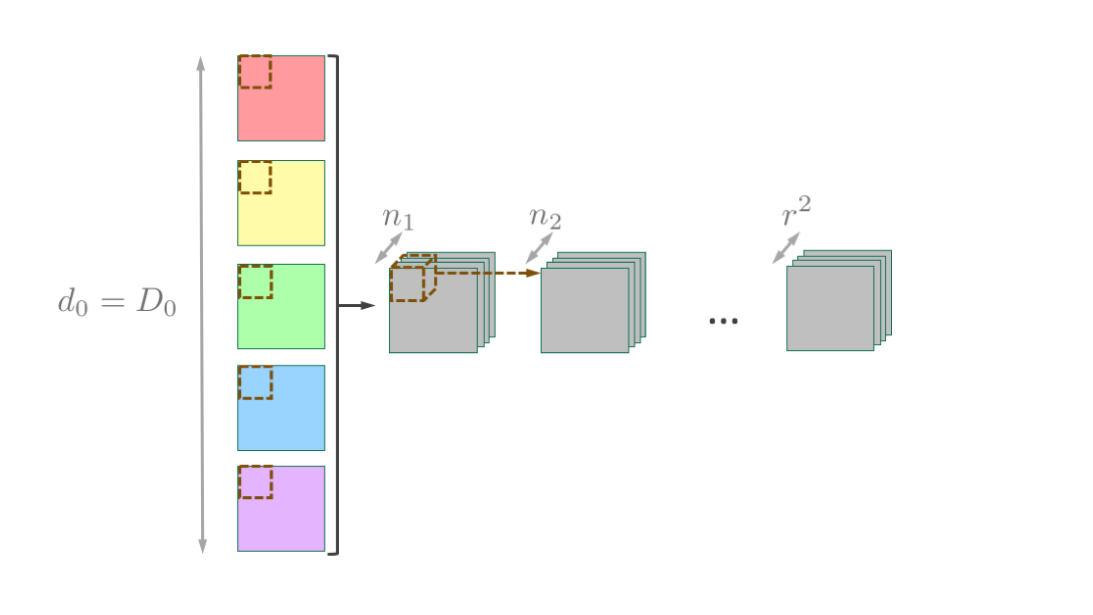
\includegraphics[width=.7\linewidth,keepaspectratio]{figures/neural_networks/early_fusion.png}
        \caption{Early fusion.}\label{subfig:earlyfus}
    \end{subfigure}
    \vskip\baselineskip
    \begin{subfigure}[b]{\subfigwidth}
        \centering
        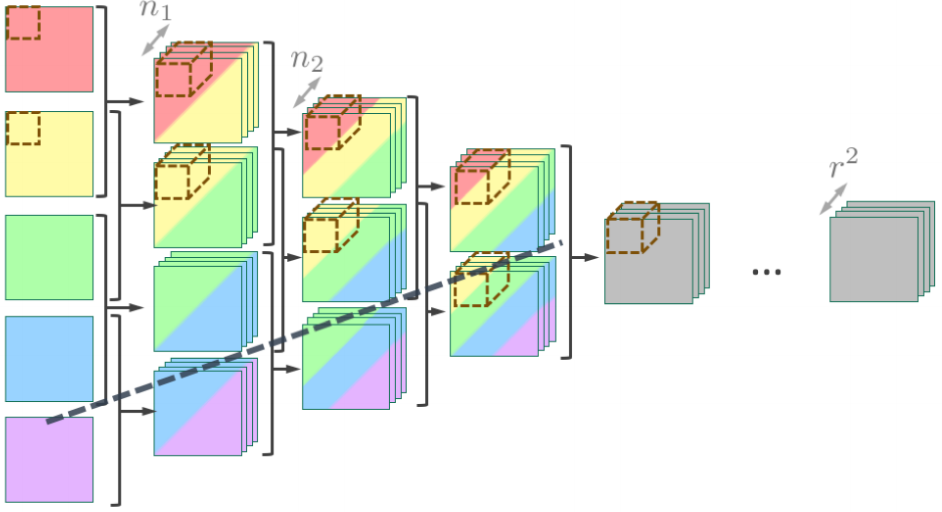
\includegraphics[width=\linewidth,keepaspectratio]{figures/neural_networks/slow_fusion.png}
        \caption{Slow fusion. If frames are processed in an online fashion then filter values should be shared. For example the last frame (purple) can recycle all of the computations above the dotted line.}\label{subfig:slowfus}
    \end{subfigure}
    % \vskip\baselineskip
    % \begin{subfigure}[b]{\subfigwidth}
    %     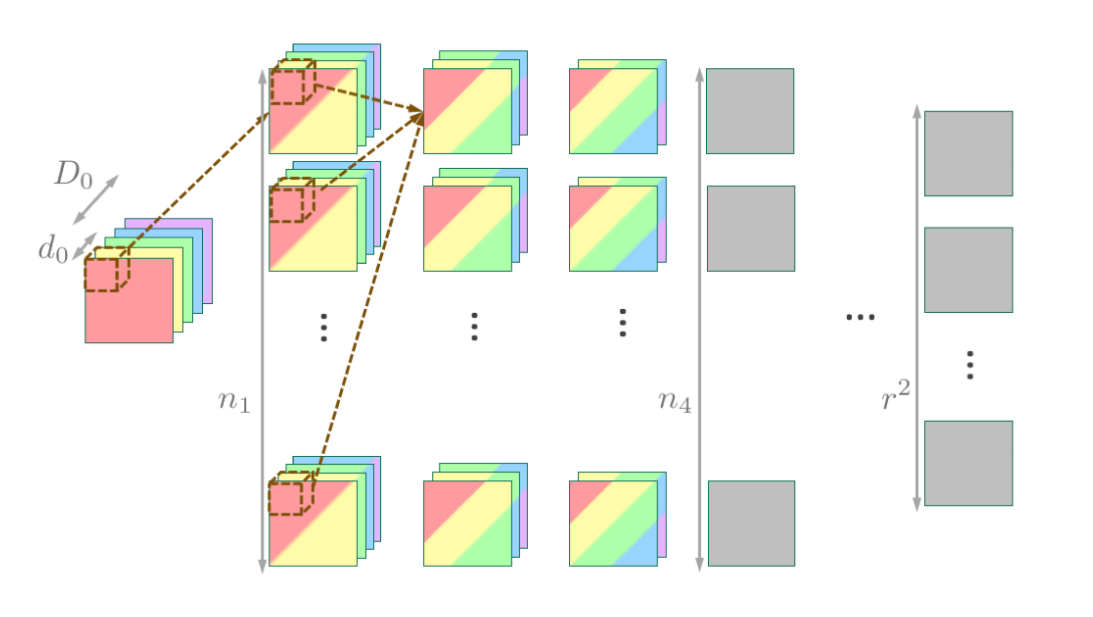
\includegraphics[width=\linewidth,keepaspectratio]{figures/neural_networks/3d_conv.png}
    %     \caption{3D convolution.}\label{subfig:updowndbpn}
    % \end{subfigure}
    \caption{Spatio-temporal ESPCN \cite{caballero2017real}.}\label{fig:fusions}
\end{figure}